\section{Data Source}
\label{sec:data_source}

\subsection{Origin of the dataset}
The competition provides two files in Apache Parquet format:

\begin{table}[H]
\centering
\caption{Competition data files.}
\begin{tabular}{lll}
\toprule
\textbf{File} & \textbf{Rows} & \textbf{Description} \\
\midrule
\texttt{train.parquet} & 5,337,414 & Training data with targets \\
\texttt{test.parquet} & --- & Test data (targets hidden) \\
\bottomrule
\end{tabular}
\end{table}

Each row in the training data contains:

\begin{table}[H]
\centering
\caption{Column schema for \texttt{train.parquet}.}
\label{tab:schema}
\begin{tabular}{lll}
\toprule
\textbf{Column} & \textbf{Type} & \textbf{Description} \\
\midrule
\texttt{code} & Categorical & Entity identifier (23 unique codes) \\
\texttt{sub\_code} & Categorical & Sub-entity identifier \\
\texttt{sub\_category} & Categorical & Category label \\
\texttt{horizon} & Integer & Forecast horizon (4 unique: 1, 5, 10, 22) \\
\texttt{ts\_index} & Integer & Temporal index (not calendar dates) \\
\texttt{y\_target} & Float & Target variable to forecast \\
\texttt{weight} & Float & Observation-level weight for scoring \\
\texttt{x0}--\texttt{x85} & Float & 86 anonymized predictor features \\
\bottomrule
\end{tabular}
\end{table}

\subsubsection{Panel Structure}

A unique time series is identified by the tuple \texttt{(code, sub\_code, sub\_category, horizon)}. The dataset contains \textbf{36,923 unique series} in total, with varying lengths. The integer-indexed \texttt{ts\_index} provides temporal ordering without revealing calendar information.

The four forecast horizons---1, 5, 10, and 22---suggest daily financial data with horizons corresponding to 1 day, 1 week, 2 weeks, and approximately 1 month of trading days.

\subsubsection{Anonymization}

All identifiers are anonymized (e.g., \texttt{MRV5UON2}, \texttt{KL66VIS3}, \texttt{V8BKY1IV}), and the 86 predictor features are labeled generically as \texttt{x0} through \texttt{x85}. This design prevents domain-specific shortcuts and forces participants to rely purely on statistical methodology.

\subsection{Data Characteristics}
The training dataset (\texttt{train.parquet}) consists of \textbf{5,337,414 rows} spanning 36,923 unique time series. Each series is uniquely identified by the four-tuple \texttt{(code, sub\_code, sub\_category, horizon)}.

\subsubsection{Dimensionality}

\begin{table}[H]
\centering
\caption{Dataset dimensionality summary.}
\begin{tabular}{lr}
\toprule
\textbf{Attribute} & \textbf{Value} \\
\midrule
Total rows & 5,337,414 \\
Total unique series & 36,923 \\
Unique codes & 23 \\
Unique horizons & 4 (1, 5, 10, 22) \\
Predictor features & 86 (\texttt{x0}--\texttt{x85}) \\
\bottomrule
\end{tabular}
\end{table}

\subsubsection{Series Length Distribution}

Series lengths vary considerably across the panel. The \texttt{ts\_index} column serves as an integer timestamp, with values ranging from early indices to several thousand. This heterogeneity in series length is a critical challenge: some series have thousands of observations, while others have fewer than 100.

The distribution of series lengths is right-skewed, with a long tail of very long series and a substantial mass of short series. This has direct implications for model selection---classical models requiring many observations (e.g., SARIMA with seasonal components) will be ineligible for short series.

\subsection{Target Variable: \texttt{y\_target}}

The target variable \texttt{y\_target} represents anonymized financial returns or derived quantities. Key distributional properties include:

\begin{itemize}
    \item \textbf{Near-zero median:} The median of \texttt{y\_target} across all observations is approximately zero, consistent with efficient-market returns.
    \item \textbf{Heavy tails:} The distribution exhibits significant excess kurtosis (leptokurtic), with extreme values far exceeding what a Gaussian model would predict. This is a hallmark of financial data.
    \item \textbf{Approximate symmetry:} The distribution is roughly symmetric around zero, though slight skewness exists in some sub-panels.
\end{itemize}

The heavy-tailed nature of the target has important modeling consequences:
\begin{enumerate}
    \item Standard squared-error loss functions will be heavily influenced by outliers.
    \item Robust loss functions or outlier-aware training procedures may be necessary.
    \item The weighted skill score metric amplifies this effect through the weight column.
\end{enumerate}

\subsection{Weight Distribution}
\label{sec:weight_dist}

The \texttt{weight} column determines each observation's contribution to the competition metric. The weight distribution exhibits \textbf{extreme concentration}:

\begin{itemize}
    \item The top 1\% of rows by weight contribute approximately \textbf{65\%} of the total weighted skill score.
    \item Many observations have very small weights, contributing negligibly to the evaluation.
    \item Weight values are non-negative and continuous.
\end{itemize}

This concentration has profound implications:
\begin{enumerate}
    \item \textbf{Model optimization must be weight-aware.} Training with uniform loss ignores the scoring structure.
    \item \textbf{The weight column should be used for loss weighting during training}, not as an input feature.
    \item \textbf{Evaluation metrics must always be weighted} to reflect the true competition ranking.
\end{enumerate}

\begin{figure}[H]
\centering
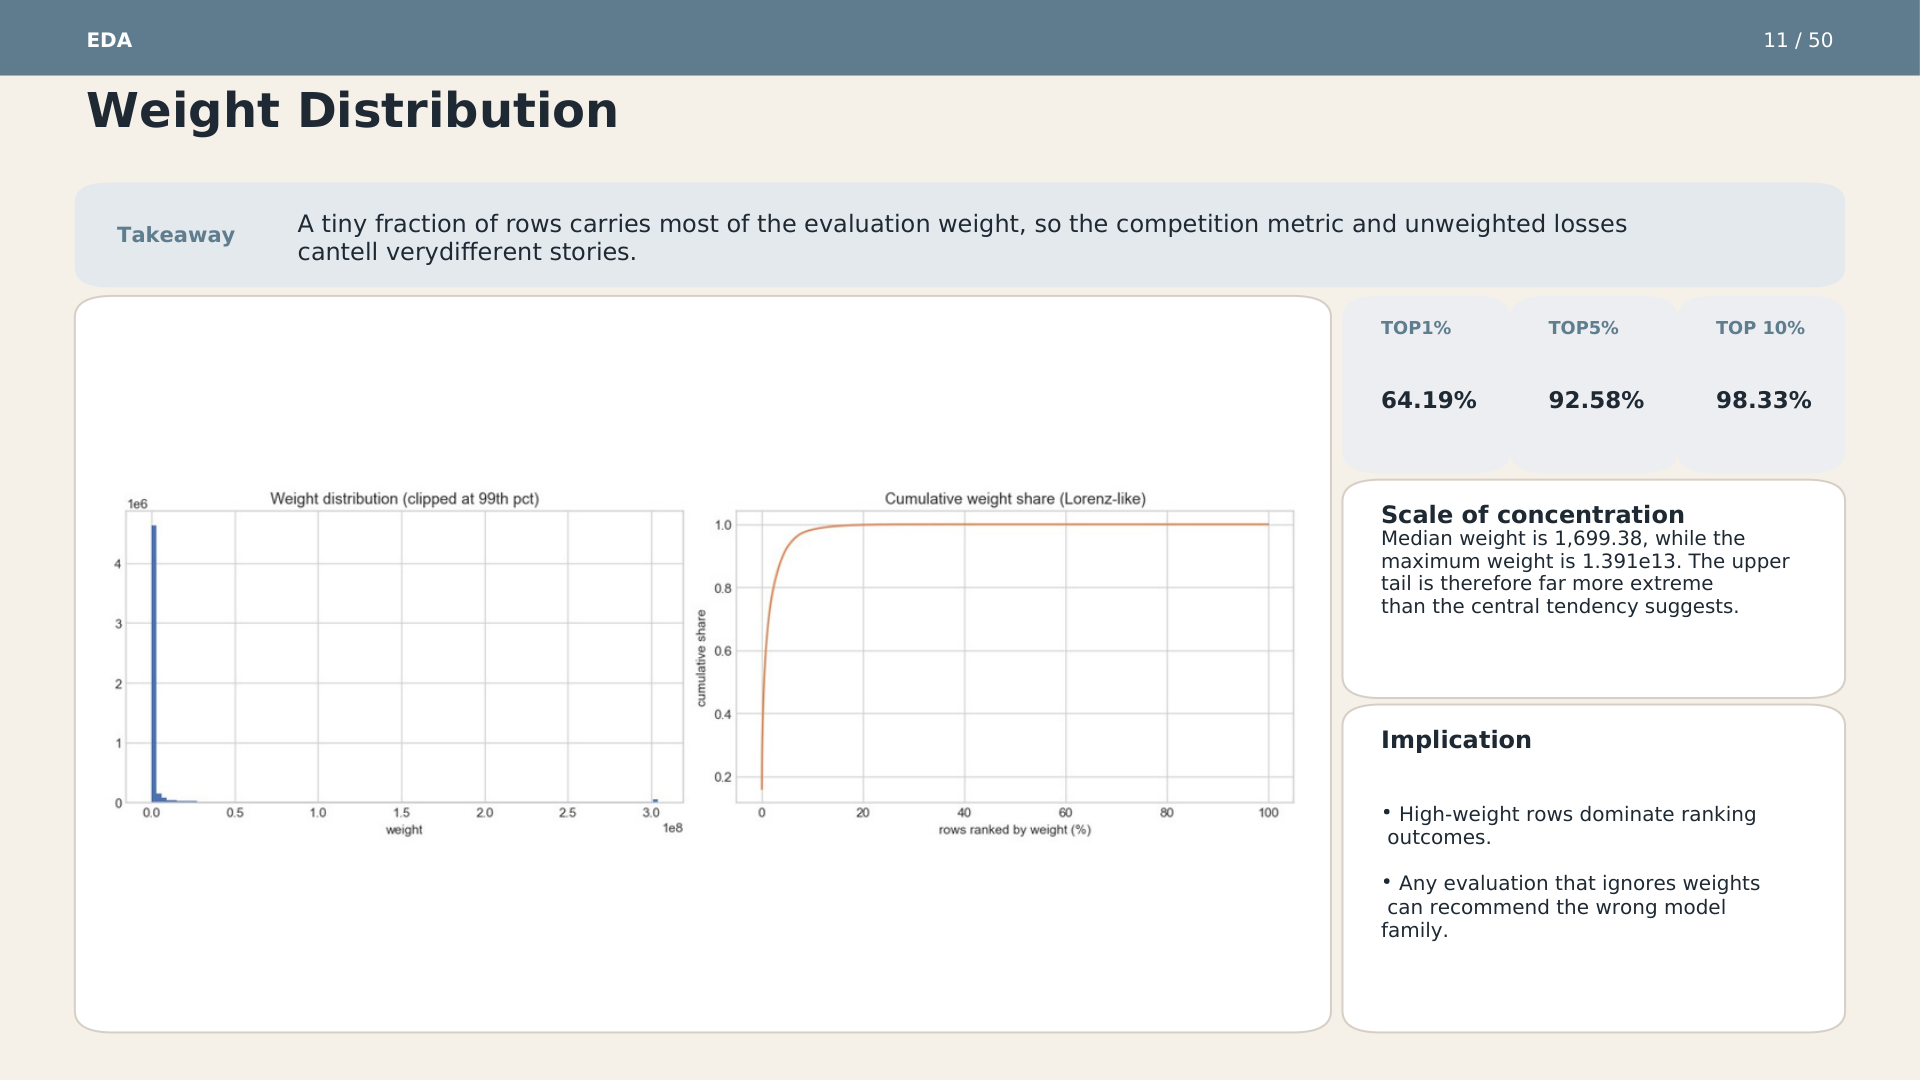
\includegraphics[width=0.95\textwidth]{figures/slide_11.png}
\caption{Weight distribution and concentration analysis. Left: weight distribution clipped at the 99th percentile shows extreme right-skew. Right: the cumulative weight share (Lorenz-like curve) reveals that the top 1\% of rows carry 64.19\% of the total weight, the top 5\% carry 92.58\%, and the top 10\% carry 98.33\%. The median weight is 1,699 while the maximum reaches $1.39 \times 10^{13}$.}
\label{fig:weight_dist}
\end{figure}

\subsection{Data Pre-processing}
The 86 anonymized predictor features are labeled \texttt{x0} through \texttt{x85}. Key findings from initial exploration:

\begin{itemize}
    \item \textbf{Weak individual correlations:} No single feature exhibits a correlation with \texttt{y\_target} exceeding $|\rho| = 0.10$. This indicates that linear univariate models using individual features will perform poorly.
    \item \textbf{Nonlinear relationships likely exist:} The weak linear correlations do not preclude strong nonlinear relationships, motivating the use of neural network models.
    \item \textbf{Feature interactions matter:} The signal likely resides in combinations of features rather than individual predictors, favoring ensemble and deep learning approaches.
\end{itemize}
Handling missing values and normalization are intrinsically tied to the feature space. The dataset contains missing values in the predictor features (\texttt{x0}--\texttt{x85}). The missingness pattern is:

\begin{itemize}
    \item \textbf{Not uniformly distributed:} Some features have significantly more missing values than others.
    \item \textbf{Potentially informative:} The pattern of missingness may itself carry signal (e.g., certain features may be unavailable for specific entity types).
    \item \textbf{Handling strategy:} For classical univariate models, missing features are irrelevant since only \texttt{y\_target} is used. For deep learning models, imputation or masking strategies are required.
\end{itemize}

\subsection{Exploratory Analysis}
\subsubsection{Global Distribution}

The global distribution of \texttt{y\_target} across all 5.3 million observations exhibits:

\begin{itemize}
    \item \textbf{Central tendency:} Mean $\approx 0$, median $\approx 0$
    \item \textbf{Dispersion:} Standard deviation varies significantly across series
    \item \textbf{Tail behavior:} Excess kurtosis $\gg 3$ (heavy tails)
    \item \textbf{Outliers:} Extreme values exist, with some observations many standard deviations from the mean
\end{itemize}

The near-zero mean and median are consistent with financial returns in an efficient market, where expected returns on short horizons are close to zero after adjusting for risk.

\begin{figure}[H]
\centering
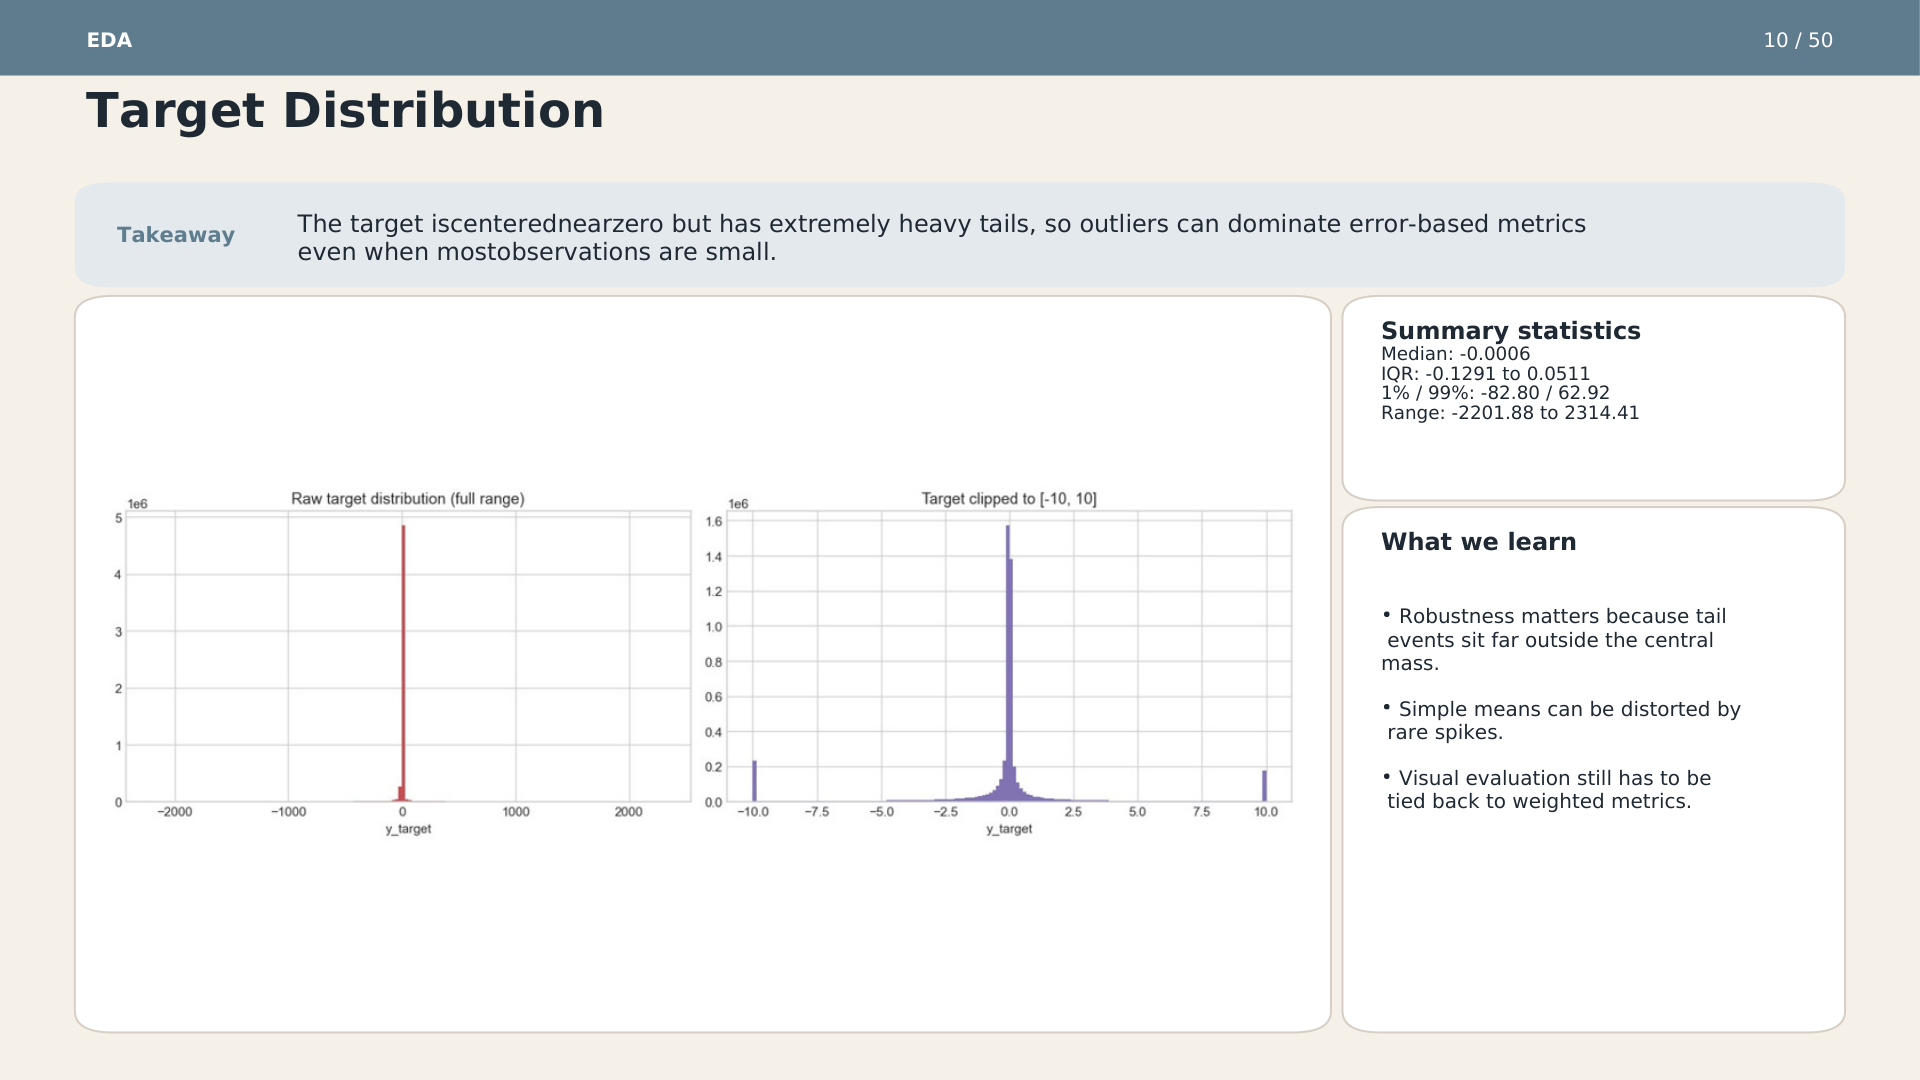
\includegraphics[width=0.95\textwidth]{figures/slide_10.png}
\caption{Target distribution analysis. Left: raw target distribution showing extreme heavy tails (range: $-2201$ to $+2314$). Right: target clipped to $[-10, 10]$ revealing the sharp central peak near zero. Summary statistics: median $= -0.0006$, IQR $= [-0.13, 0.05]$.}
\label{fig:target_dist}
\end{figure}

\subsubsection{Per-Horizon Distribution}

Decomposing by forecast horizon reveals that:
\begin{itemize}
    \item Horizon 1 (1-day) series tend to have smaller absolute values and tighter distributions.
    \item Longer horizons (10, 22) exhibit greater dispersion, consistent with the square-root-of-time scaling of volatility.
\end{itemize}

\subsection{Stationarity Analysis}
\label{sec:stationarity}

Stationarity is a fundamental assumption underlying most classical time series models. We test stationarity using the \textbf{Augmented Dickey-Fuller (ADF) test} on eligible series.

\subsubsection{ADF Test on Levels}

Applying the ADF test to the raw \texttt{y\_target} series (levels) at the 5\% significance level:
\begin{itemize}
    \item A substantial fraction of series reject the null hypothesis of a unit root, suggesting stationarity in levels.
    \item However, many series fail to reject, indicating non-stationarity.
\end{itemize}

\subsubsection{ADF Test on First Differences}

After first differencing ($\Delta y_t = y_t - y_{t-1}$):
\begin{itemize}
    \item \textbf{100\% of eligible series become stationary} at the 5\% significance level.
    \item This is the single most consequential finding of the EDA.
\end{itemize}

\begin{figure}[H]
\centering
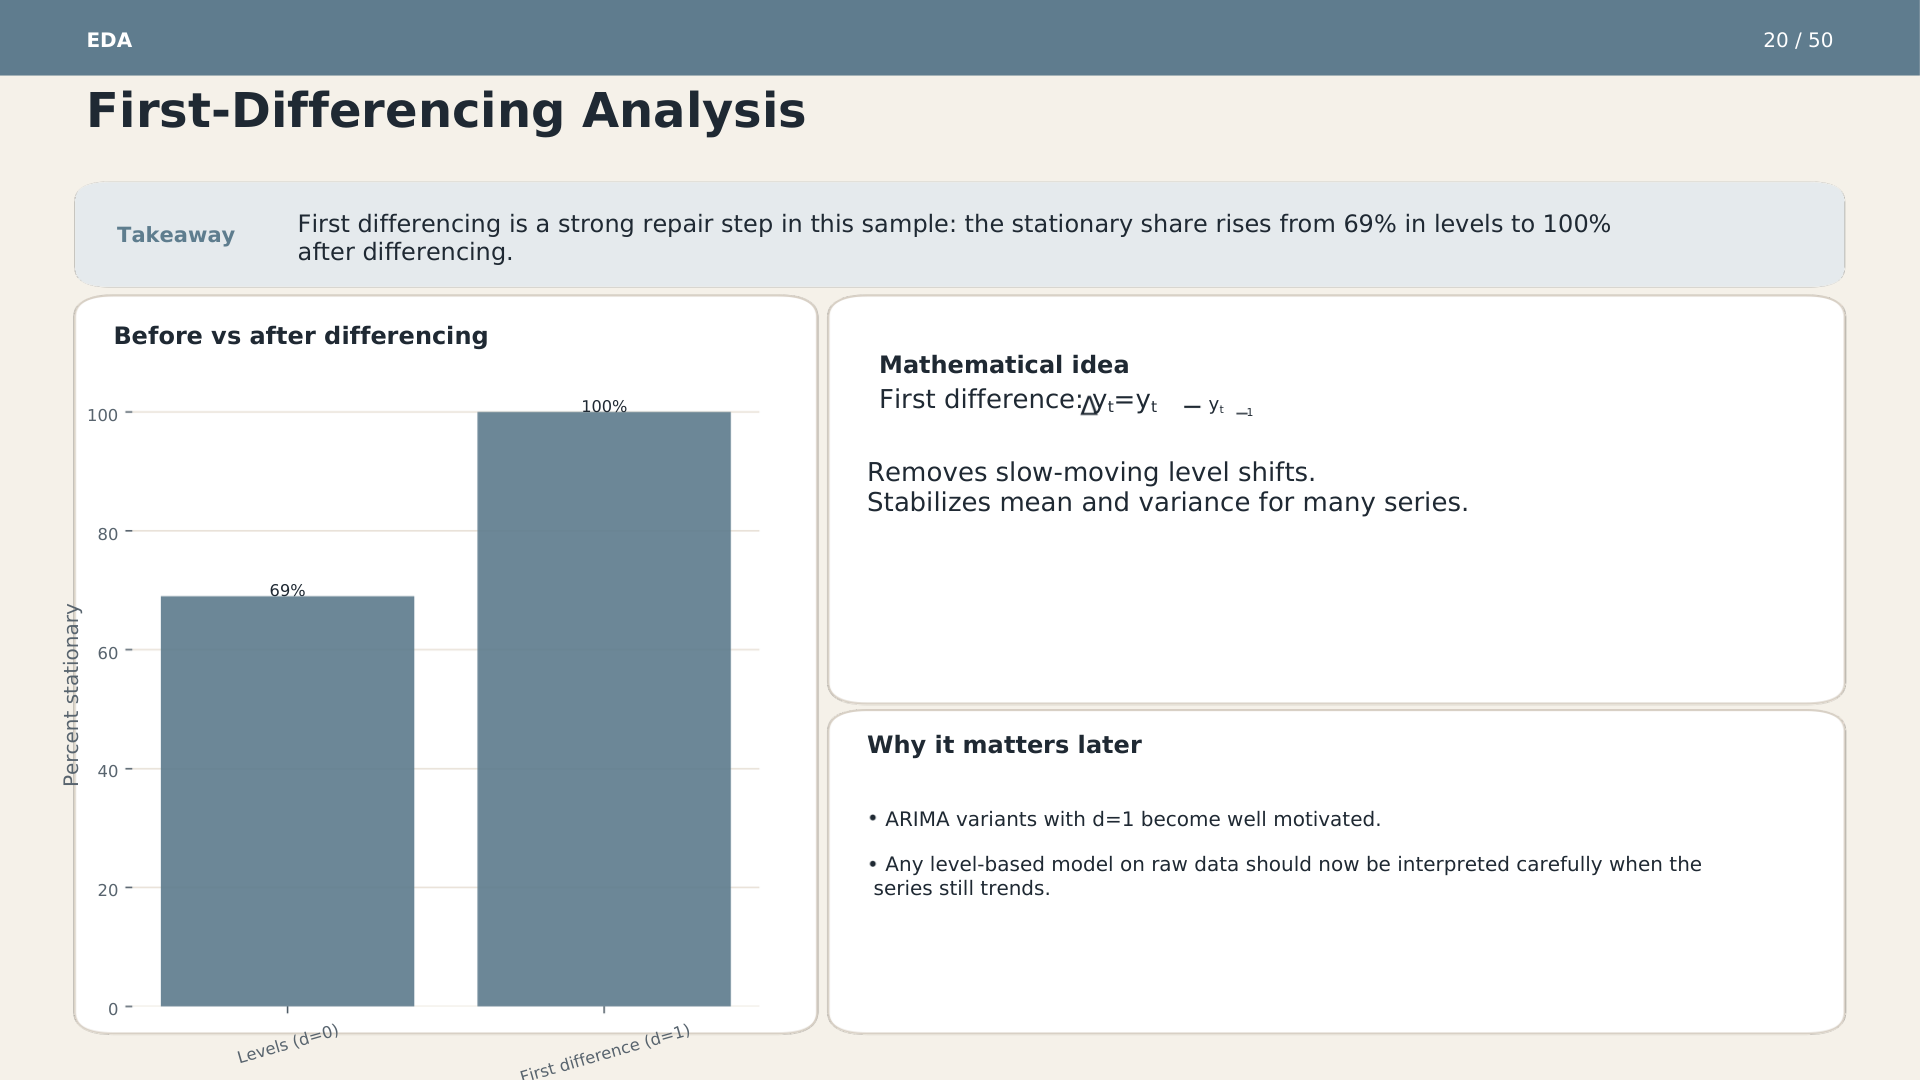
\includegraphics[width=0.95\textwidth]{figures/slide_20.png}
\caption{First-differencing analysis. Before differencing, 69\% of series are stationary; after first differencing ($\Delta y_t = y_t - y_{t-1}$), 100\% achieve stationarity. This result directly motivates using $d=1$ in all ARIMA-family models.}
\label{fig:stationarity}
\end{figure}

This result directly shapes the classical modeling strategy: every parametric model either fits on first differences explicitly (AR, MA, ARMA families) or uses $d = 1$ within the ARIMA/SARIMA framework.

\subsection{Autocorrelation Structure}

\subsubsection{ACF and PACF Analysis}

The autocorrelation function (ACF) and partial autocorrelation function (PACF) reveal the temporal dependence structure:

\begin{itemize}
    \item \textbf{Panel-level ACF:} The top lags with significant autocorrelation are short---lags 1, 2, and 3 dominate. This suggests that AR and MA orders of $p, q \in \{1, 2, 3\}$ should capture most of the serial structure.
    \item \textbf{Rapid decay:} Autocorrelations decay quickly, consistent with near-efficient financial markets where predictable structure is quickly arbitraged away.
    \item \textbf{No panel-wide seasonality:} The ACF at seasonal lags (7, 24, etc.) does not show systematic peaks across the panel.
\end{itemize}

\subsubsection{Implications for Model Order Selection}

The ACF/PACF analysis motivates the following model order choices:
\begin{itemize}
    \item AR orders: $p = 1, 2, \ldots, 10$ (with most signal expected at low orders)
    \item MA orders: $q = 1, 2, \ldots, 10$ (mirroring the AR scan)
    \item ARMA combinations: Selected $(p, q)$ pairs with total order $p + q \leq 8$
\end{itemize}

\subsection{Cross-Correlation Analysis}

The correlation between each predictor feature (\texttt{x0}--\texttt{x85}) and the target \texttt{y\_target} is uniformly weak:

\begin{itemize}
    \item All Pearson correlations satisfy $|\rho| < 0.10$.
    \item This implies that \textbf{no single feature is a strong linear predictor} of the target.
    \item Multivariate and nonlinear models (gradient-boosted trees, neural networks) are necessary to exploit any feature-based signal.
\end{itemize}

This finding is consistent with the efficient-market hypothesis in quantitative finance: if a single observable feature were strongly predictive of returns, it would be quickly arbitraged away.

\subsection{Weight Concentration Analysis}

As introduced in Section~\ref{sec:weight_dist}, the weight distribution is highly concentrated. The EDA quantifies this precisely:

\begin{itemize}
    \item \textbf{Top 1\% of rows:} $\sim$65\% of total weighted score
    \item \textbf{Top 10\% of rows:} $\sim$90\% of total weighted score
    \item \textbf{Bottom 50\% of rows:} $<$5\% of total weighted score
\end{itemize}

This extreme concentration means that model performance on a small number of high-weight observations overwhelmingly determines the competition score. A model that performs well on high-weight observations but poorly on low-weight ones will substantially outperform a model that is uniformly mediocre.

\subsection{STL Decomposition}

\textbf{STL (Seasonal-Trend decomposition using LOESS)} decomposes each series into three additive components:

\begin{equation}
y_t = T_t + S_t + R_t
\end{equation}

where $T_t$ is the trend, $S_t$ is the seasonal component, and $R_t$ is the residual.

\subsubsection{Period Detection via ACF}

Before running STL, we detect the dominant period for each series using the ACF. The procedure:
\begin{enumerate}
    \item Compute the ACF up to 100 lags.
    \item Identify the top 10 peaks (excluding lag 0).
    \item Select the strongest peak with lag $\geq 2$ as the candidate period.
\end{enumerate}

\subsubsection{Decomposition Findings}

Applying STL to representative series (anchored to the longest-history series for consistency with the ACF/PACF analysis):

\begin{itemize}
    \item \textbf{Trend:} Most series exhibit a non-trivial trend component, confirming non-stationarity in levels (consistent with the ADF results).
    \item \textbf{Seasonal:} The seasonal component amplitude is typically small relative to the observed range, confirming the absence of strong panel-wide seasonality.
    \item \textbf{Residual:} Residuals often retain some structure (not pure white noise), suggesting that STL alone does not capture all temporal dynamics---motivating the use of parametric and deep learning models.
\end{itemize}

\begin{figure}[H]
\centering
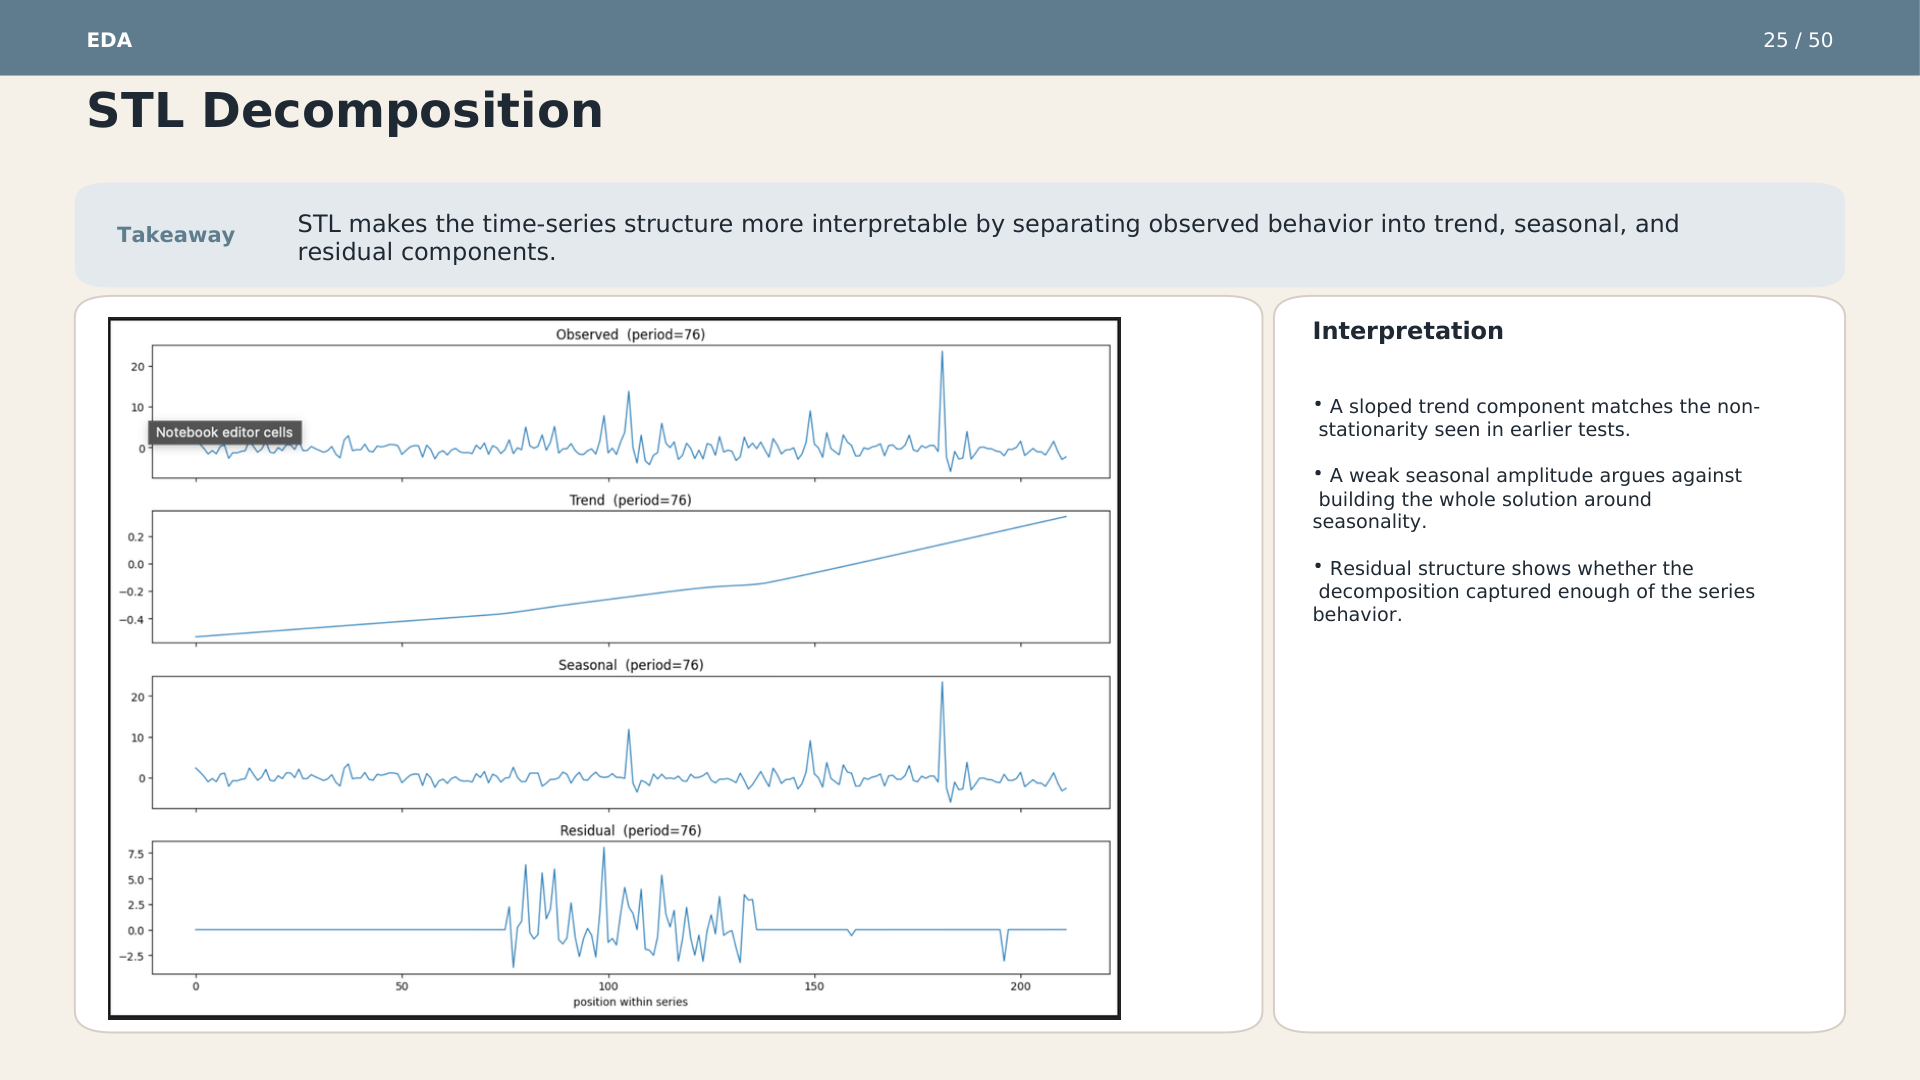
\includegraphics[width=0.95\textwidth]{figures/slide_25.png}
\caption{STL decomposition (period=76) for a representative series. The decomposition separates observed behavior into trend, seasonal, and residual components. The sloped trend confirms non-stationarity; the weak seasonal amplitude argues against building models around seasonality; residual structure indicates that additional modeling is needed.}
\label{fig:stl}
\end{figure}

\subsection{EDA Summary}
\begin{table}[H]
\centering
\caption{Summary of EDA findings and their modeling consequences.}
\label{tab:eda_summary}
\begin{tabularx}{\textwidth}{>{\raggedright\arraybackslash}p{4cm}>{\raggedright\arraybackslash}p{4cm}>{\raggedright\arraybackslash}X}
\toprule
\textbf{Finding} & \textbf{EDA Section} & \textbf{Modeling Consequence} \\
\midrule
Heavy-tailed target, median $\approx 0$ & \S4 & Include Zero as a baseline; the skill-score denominator is the zero-forecast error \\
\addlinespace
Weight concentration: top 1\% $\to$ 65\% of score & \S5 & Never report unweighted metrics; all leaderboards use weighted metrics \\
\addlinespace
Only $\sim$1,930 series cross VAL\_CUTOFF & \S6 & Evaluate only eligible series \\
\addlinespace
Weak per-feature correlations ($|\rho| < 0.10$) & \S7 & Classical univariate methods cannot exploit features; ensemble/deep models required \\
\addlinespace
100\% stationary after first differencing & \S11 & Every parametric model uses $d = 1$ \\
\addlinespace
Top ACF lags are short (1, 2, 3) & \S14 & AR/MA orders focus on $p, q \in \{1, \ldots, 10\}$ \\
\addlinespace
No panel-wide seasonality & \S14--15 & SARIMA included for completeness, not expected to win \\
\bottomrule
\end{tabularx}
\end{table}

